\subsection{Study B: controlled evidence availability}

Study A's coverage gap motivated a separate follow-up after its outcomes were known. We retained the byte-identical world, controllers, and evaluator, then froze a new complete factorial grid before collecting its own data. Source commit \texttt{\seqsplit{d805b3e3560c05ee0a7efd02a80fc18503c6ee05}}, protocol commit \texttt{\seqsplit{b937920469285cdd971783fa6cb33216a7e4da13}}, and protocol SHA-256 \texttt{\seqsplit{e874c6781aa0dbc8ef682ea0a8d37c25d73cc861dada05fd0379116d4a7f6584}} bind that design. This is a disclosed, post hoc motivated sensitivity experiment, rather than a new held-out corpus or replacement for Study A.

The 64 profiles cross readback lag $\{0,40,80,95\}$ ms with independently varied unavailable-until and incomplete-until times $\{0,170,210,250\}$ ms. Each profile repeats in the three domains at seed zero: 192 cases and 960 scheduled policy worlds. Here $D=100$, $H=150$, $R=250$, and $S=330$ ms; reads remain at $50,150,190,230$ ms. Every initial dispatch acknowledges at 2 ms and creates one correct effect at 10 ms. All arms share native idempotency. There are no external writes, removals, or wrong effects. This intentionally uniform physical-success design isolates evidence-window coverage and cost. Profiles are controlled mechanisms, and the three domains repeat them; neither 192 cases nor 960 worlds represent independent task samples.

All 960 worlds completed without failure. The separately implemented auditor verified 1,925 saved artifacts, queried all 960 SQLite snapshots, and agreed with the summary. Unlike Study A, the original collector produced its terminal manifest and receipt normally. All five policies dispatched once, achieved original and recovery satisfaction in 192/192 worlds, and had zero duplicate or unwanted events. Their physical effect histories agreed in every five-arm case. Thus the primary safe-recovery contrast is zero.

\begin{table*}[t]
\caption{Study B: exact finite-grid reports and read costs, 192 planned/completed worlds per policy. Every definite report is hindsight-correct in this uniform-success design. It cannot estimate the response policy's false-success risk. Linked abstention is distinct from state abstention.}
\label{tab:availability-results}
\centering\small
\setlength{\tabcolsep}{4pt}
\begin{tabular}{lrrrrr}
\toprule
Policy & State correct/planned & State unknown & Linked correct/planned & Total reads & Mean decision (ms) \\
\midrule
Response retry & 192/192 & 0/192 & 192/192 & 0 & 2 \\
Readback state & 81/192 & 111/192 & 0/192 & 741 & 224.375 \\
Separate reference & 81/192 & 111/192 & 81/192 & 741 & 224.375 \\
ConseqaX one final read & 3/192 & 189/192 & 3/192 & 192 & 150 \\
ConseqaX polling & 81/192 & 111/192 & 81/192 & 741 & 224.375 \\
\bottomrule
\end{tabular}
\end{table*}

The one-final-read policy resolved one of 64 profiles per domain; polling resolved 27, matching the prospectively specified timing calculation. The paired correct-state-yield increase is $78/192=26/64=0.40625$, shared by the reference and state-only readback. All 192 reference--polling pairs agreed on reports, endpoint vectors, dispatch decisions, and physical records. State-only differed from polling in 81 linked reports while preserving actions and physical outcomes. Polling used 741 reads versus 192 for one-final-read, or 3.859375 versus one per world; mean logical decision time increased by 74.375 ms. These are charged simulated reads and decision times, not production latency.

The full factor grid in Fig.~\ref{fig:availability-grid} shows the boundary: late opportunities help only when availability and completeness recover and the watermark reaches $H$. Lag 95 ms and either window persisting through 250 ms remain unresolved. The ACK-driven response policy reports all 192 successes correctly in hindsight with no read, since all effects are constructed to succeed. Its report arrives before the effect and without horizon-covering evidence; this experiment supplies no estimate of its risk in failing worlds. Together, the studies show conditional polling utility and its cost, with no package superiority over the equally informed reference, no additional recovery-action benefit, and no task-population inference.

\begin{figure*}[p]
\centering
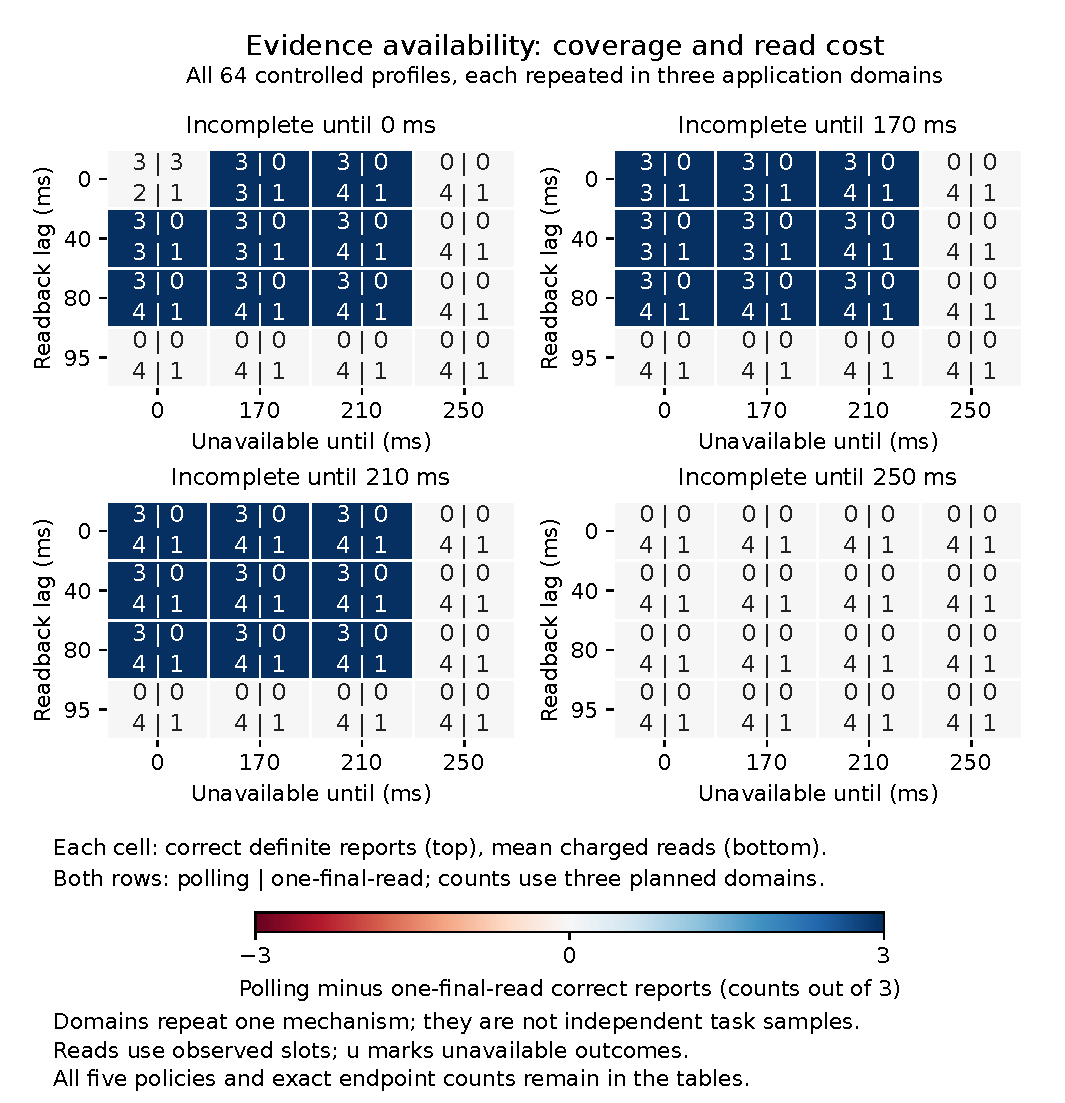
\includegraphics[width=\textwidth,height=0.76\textheight,keepaspectratio]{recovery-availability-grid.pdf}
\caption{Study B: all 64 controlled availability profiles, repeated across three domains. Actual report coverage and read costs are retained for polling and one-final-read. These paired conditions isolate evidence timing; every policy has identical successful physical outcomes, and the classical reference matches polling.}
\label{fig:availability-grid}
\end{figure*}
